% Previous work into shearing bijels have demonstrated how particles prefer to move in the direction of shear and if strong enough, even detach from the interface. \cite{bonaccorso_shear_2020} It has also been shown how at curved interfaces, ellipsoidal particles  

\section{Introduction}

The rheological properties of bijels are critical to their processability and structural fidelity across a variety of manufacturing techniques. In solvent transfer-induced phase separation 
(STrIPS), for example, the flow rate of the casting mixture and the co-solvent ratio play a key role in controlling the microstructure of the bijel and determining whether droplets or 
rope-like structures emerge during synthesis \cite{haase_continuous_2015, haase_situ_2016}. Similarly, in volatile-induced phase separation (VIPS), the viscosity of the solvent rich and poor 
phases determines the extent of phase separation before gelation or jamming occurs, ultimately governing final domain morphology \cite{wang_scalable_2020}. In homogenization-driven methods, 
the imposed shear rate directly influences the interfacial jamming dynamics and can either assist or disrupt bicontinuous structure formation depending on processing windows 
\cite{huang_bicontinuous_2017}. Understanding these rheological dependencies is essential for tuning bijel architectures for advanced applications.

While the microstructure and synthesis of bijels have been extensively investigated, their rheological behaviour remains comparatively underexplored. One intriguing feature is the formation of 
monogels, in which remixing the liquid phases of a bijel preserves the interfacial particle network due to persistent attractive interactions between particles \cite{sanz_colloidal_2009}. This 
phenomenon has been observed in bijels composed of lutidine/water and styrene/butadiene oligomer mixtures, but is notably in systems based on ethylene glycol and nitromethane 
\cite{sanz_colloidal_2009, bai_dynamics_2015, tavacoli_novel_2011}. Rheologically, bijels typically exhibit shear thinning and thixotropic responses under steady shear, indicative of dynamic 
restructuring and gradual recovery of the internal network \cite{macmillan_rheological_2019}. In confined geometries, computational studies have shown that shear induces elongation 
of domains followed by particle alignment along the flow direction, detachment from the interface, and eventual collapse of the bicontinuous structure \cite{bonaccorso_shear_2020}. More recently, 
bijels have been conceptualized as two-dimensional colloidal glasses embedded in a percolating three-dimensional network, exhibiting rheological behaviour that bridges colloidal gels and jammed 
particle layers \cite{ching_bijel_2022}. However, existing frameworks for bijel rheology focus on bijels stabilized by spherical, non-stimuli responsive particles, and do not yet capture the complex 
rheology arising from anisotropic particle shapes or magnetic interactions, which are increasingly relevant in functionalized bijel systems.

While the rheology of emulsions stabilized by spherical particles has been extensively characterized, ellipsoidal particles introduce additional complexity through interfacial locking and anisotropic drag, 
which can suppress coalescence and resist flow differently under shear \cite{madivala_self-assembly_2009, daware_emulsions_2015, sun_assembly_2013}. Under shear, ellipsoidal particles 
can promote shear banding, wherein particle-fluid interactions create localized variations in velocity profiles \cite{xu_relation_2013}. Furthermore, suspensions of magnetically responsive particles, 
such as ferrofluids, exhibit a pronounced increase in viscosity due to field-induced self-assembly that restricts fluid flow \cite{qiao_magnetorheological_2012}. 
Theoretical predictions and experimental observations have identified that orientational ordering of anisotropic particles in the direction of shear reduces viscosity by minimizing hydrodynamic drag and interfacial 
disruption, allowing the fluid to flow more easily along the direction of least resistance.\cite{vermant_flow-induced_2005, xu_relation_2013}. 

In this study, we investigate the rheological response of bijels stabilized by magnetically responsive ellipsoidal particles subjected to constant shear. Using a hybrid Lattice Boltzmann-Molecular Dynamics 
(LBM-MD) simulation framework, we model a binary fluid system containing suspended magnetic ellipsoids, with shear applied via Lees-Edwards boundary conditions along one axis and periodic conditions along 
the remaining boundaries. Our results show that these bijels exhibit Herschel-Bulkley-type rheology, with yield stress and shear-thinning behavior modulated by particle orientation at the interface. 
Specifically, increasing orientational ordering of ellipsoidal particles under the applied magnetic field reduces hydrodynamic resistance, resulting in lower effective viscosity and a diminished shear-thinning 
response. Furthermore, we find that the yield stress is dependent on particle shape and magnetic alignment, as magnetic stimuli alter the number and orientation of frictional contacts within the interfacial 
monolayer. These findings highlight the tunability of bijel rheology via particle morphology and magnetic field application, offering potential design pathways for adaptive and reconfigurable soft materials.


\section{Results}\label{sec:results_p3}

To probe the rheological behavior of bijels stabilized by ellipsoidal particles, we analyze their response under constant shear with particular focus on the influence of interfacial particle ordering 
and magnetic field application. The initial bijel structures are obtained from previous simulations, consisting of bicontinuous morphologies stabilized by either prolate or oblate magnetic 
ellipsoids at a particle volume fraction of $\phi_p = 0.15$, generated with and without an applied magnetic field of dimensionless strength $\bar{B} = 1$. To evaluate the combined and decoupled effects 
of field history and applied shear, we systematically vary the magnetic field configuration, yielding four distinct processing pathways: 
$\bar{B}:0 \rightarrow 0$, $\bar{B}:0 \rightarrow 1$, $\bar{B}:1 \rightarrow 0$, and $\bar{B}:1 \rightarrow 1$. These setups enable us to isolate the contributions of pre-aligned versus dynamically aligning 
particles during flow. Shear is imposed via a range of dimensionless shear capillary numbers, defined as $Ca_s = \frac{\dot{\gamma} R_s \eta_f}{\sigma}$, where $\dot{\gamma}$ is the applied shear rate, 
$R_s = 7.9$ is the equivalent spherical radius of the ellipsoids, $\eta_f$ is the dynamic viscosity of the continuous phase, and $\sigma$ is the interfacial tension. 
\cite{frijters_effects_2012, yang_capillary_2022} We explore five shear conditions spanning $Ca_s = 1 \times 10^{-4}$ to $1 \times 10^{-6}$, capturing the transition from strong deformation to 
near-equilibrium interfacial response.

\subsection{Viscosity measurement}

Particle ordering plays a critical role in determining the rheological behavior of suspensions, as aligned particles can more readily slide past one another 
under shear, delaying structural breakdown. In bijels, where particles are adsorbed at the fluid-fluid interface, this interfacial confinement may significantly 
influence the degree of slip and the onset of yielding. Prior studies have shown that bijels exhibit shear-thinning behavior consistent with Herschel-Bulkley rheology, 
indicating a non-Newtonian response governed by both interfacial structure and particle dynamics \cite{macmillan_rheological_2019}. To investigate these effects in 
the presence of magnetic fields and varying degrees of particle ordering, we apply constant shear to the bijel templates and plot the resulting time evolution of 
the shear stress, as shown in Figure~\ref{fig:stress_time}.

\begin{figure} 
    \centering 
    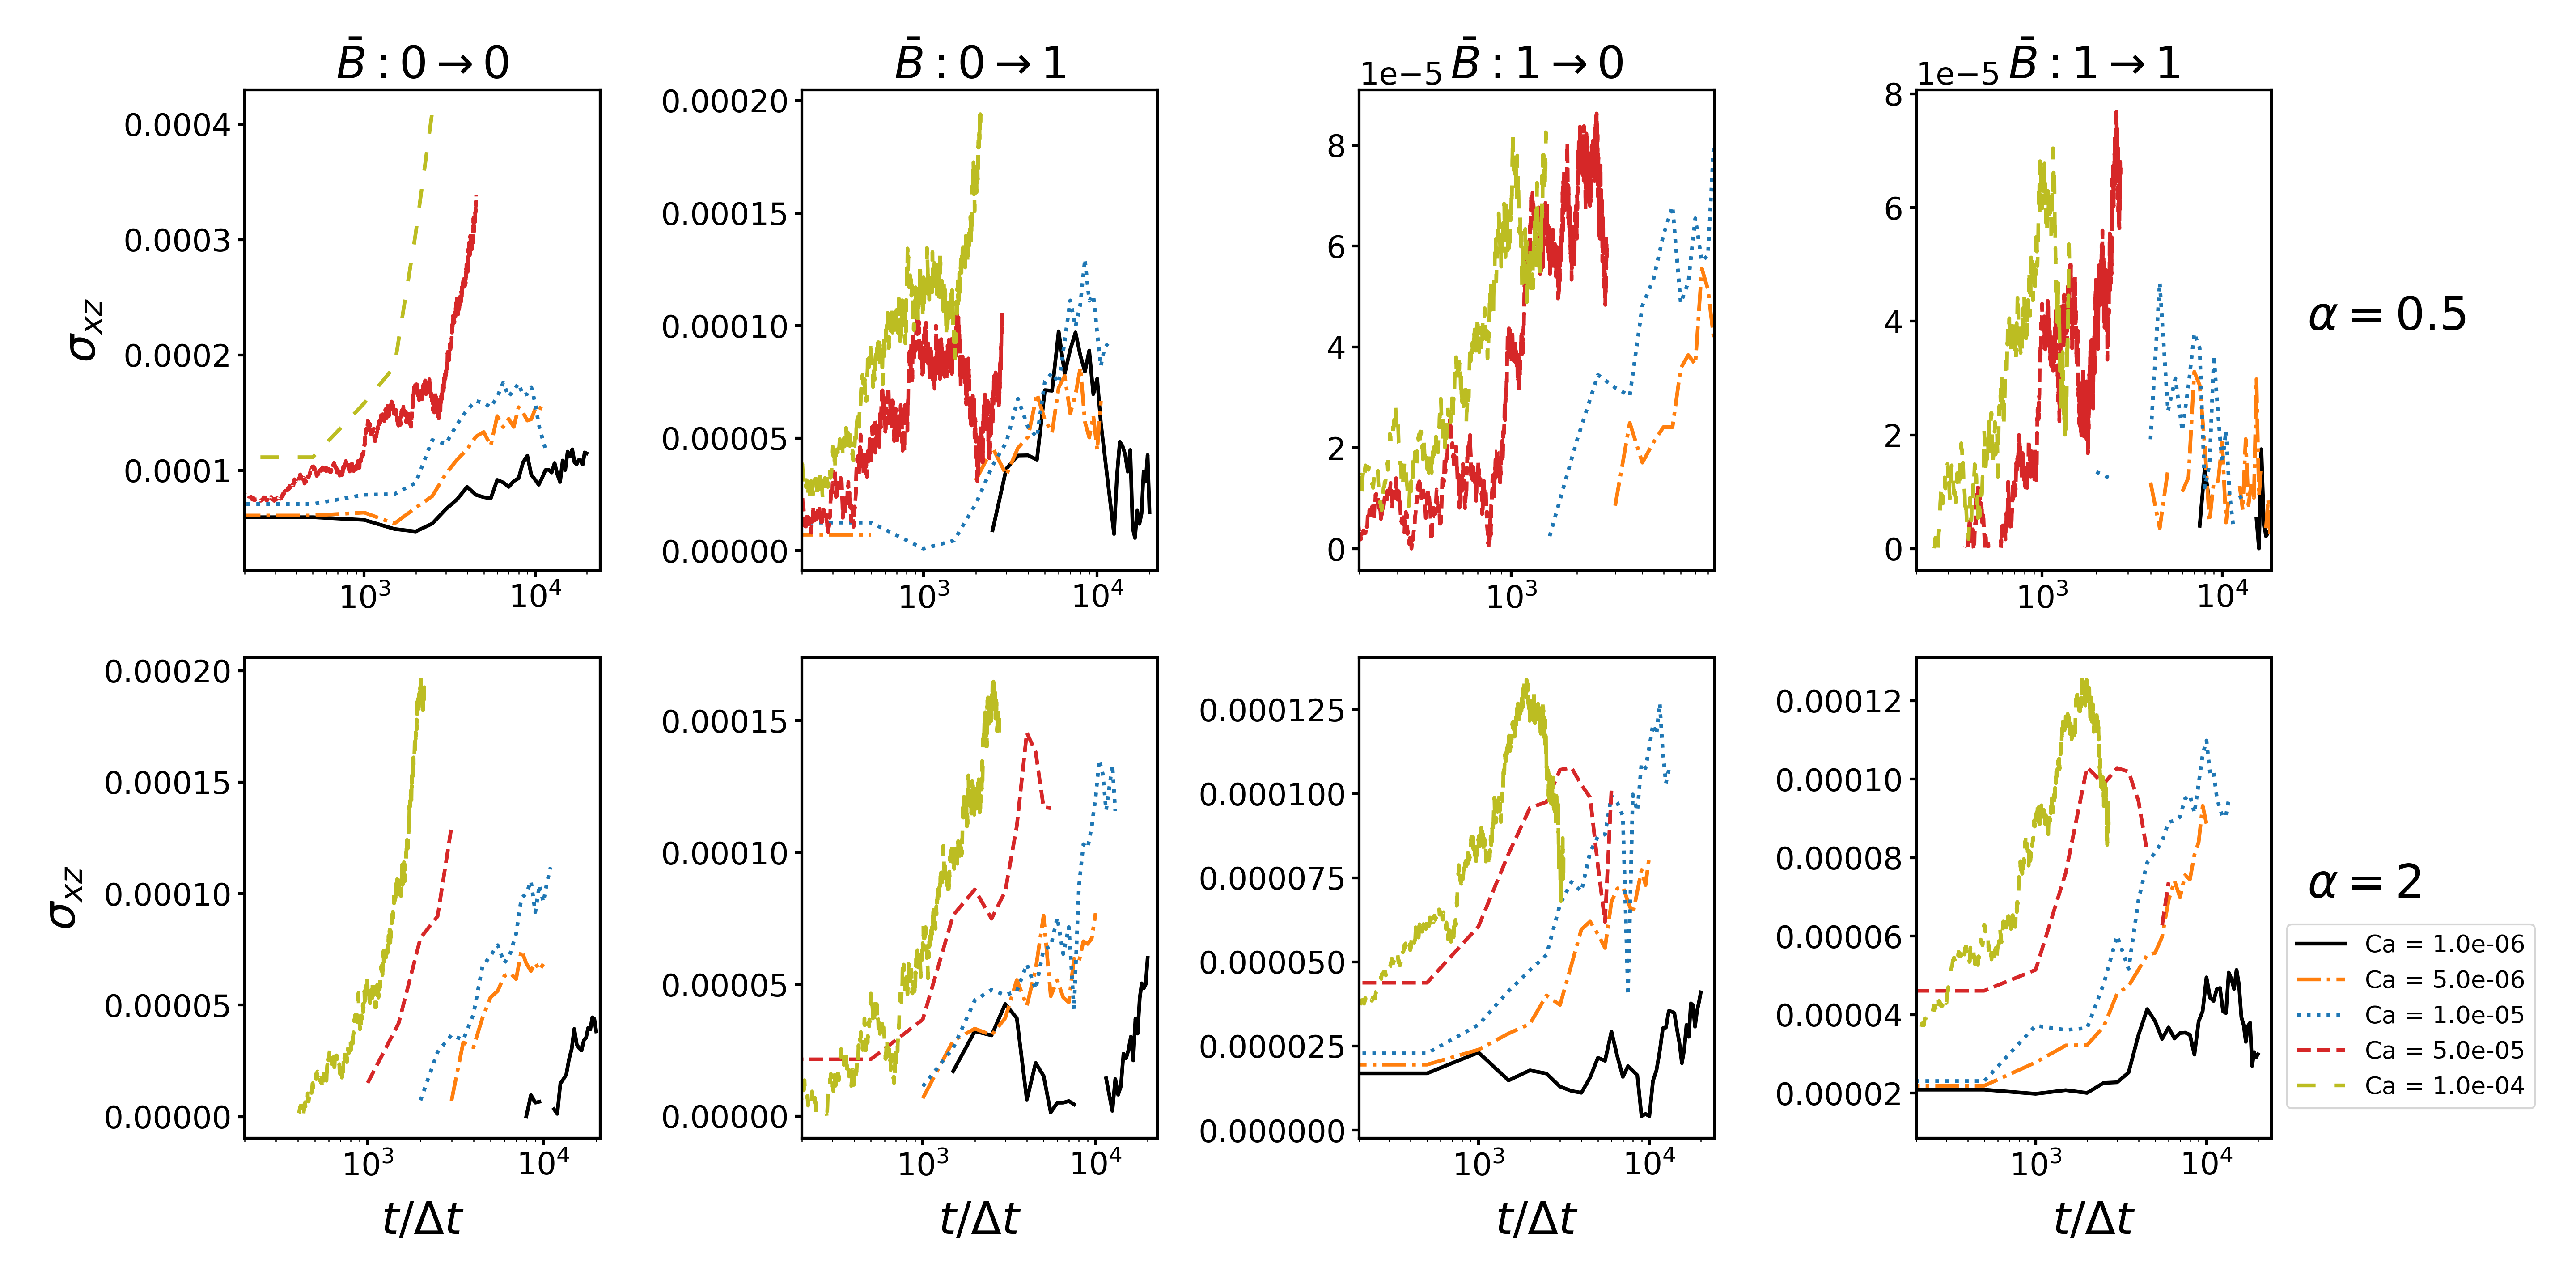
\includegraphics[scale=0.5]{../figures/results/paper3/stress-time_compare.png} 
    \caption{Time evolution of the shear stress of bijels stabilized with ellipsoidal particles as a function of the applied strain rate as
             a function of the initial microstructure and applied magnetic field. The observed stress response is difficult to say when a steady
             state is reached.} 
    \label{fig:stress_time} 
\end{figure}

Figure \ref{fig:stress_time} demonstrates that a definitive steady-state shear stress is not reached within the simulated timeframes across all conditions. 
This absence of steady-state behavior is attributed to the continued coarsening of the bicontinuous domains and the progressive reorientation of interfacial 
particles under shear \cite{tavacoli_novel_2011, macmillan_rheological_2019}. Tavacoli et al.\ showed that mechanical perturbation of bijels, such as the 
insertion of a needle to measure yield stress, resulted in irreversible structural deformation, particularly in ethanediol/nitromethane systems 
\cite{tavacoli_novel_2011}. Similarly, Macmillan et al.\ observed that repeated shearing of bijels synthesized by direct mixing led to degraded mechanical 
performance over time, suggesting a link between structural evolution and rheological response \cite{macmillan_rheological_2019}. To characterize the rheology 
of these evolving systems, we identify pseudo-steady-state regions within the stress-time profiles, defined as intervals where the rate of change of shear 
stress is minimal and persists for the longest continuous duration. Within these regions, the stress response is fitted to the applied shear rate using a 
Herschel-Bulkley model:  

\begin{equation}
    \sigma_{xz} = \sigma_{y} + K\dot{\gamma}^{n}    
\end{equation}

In the Herschel-Bulkley model, $\sigma_{xz}$ denotes the computed shear stress, $\sigma_y$ is the yield stress, $K$ represents the flow consistency index, 
and $n$ is the flow index characterizing the degree of shear thinning. In certain cases, simulations conducted at the lowest shear capillary number 
($Ca_s = 10^{-6}$) exhibited insufficient stress resolution or high variability, and were excluded from model fitting where appropriate. For each case, 
$\sigma_{xz}$ is extracted from the pseudo-steady-state region of the stres-time curves, while the corresponding shear rate $\dot{\gamma}$ is derived from 
the imposed capillary number, $Ca_s$. The resulting fits for the various bijel systems are presented in Figure~\ref{fig:stress_strain}.

\begin{figure} 
    \centering 
    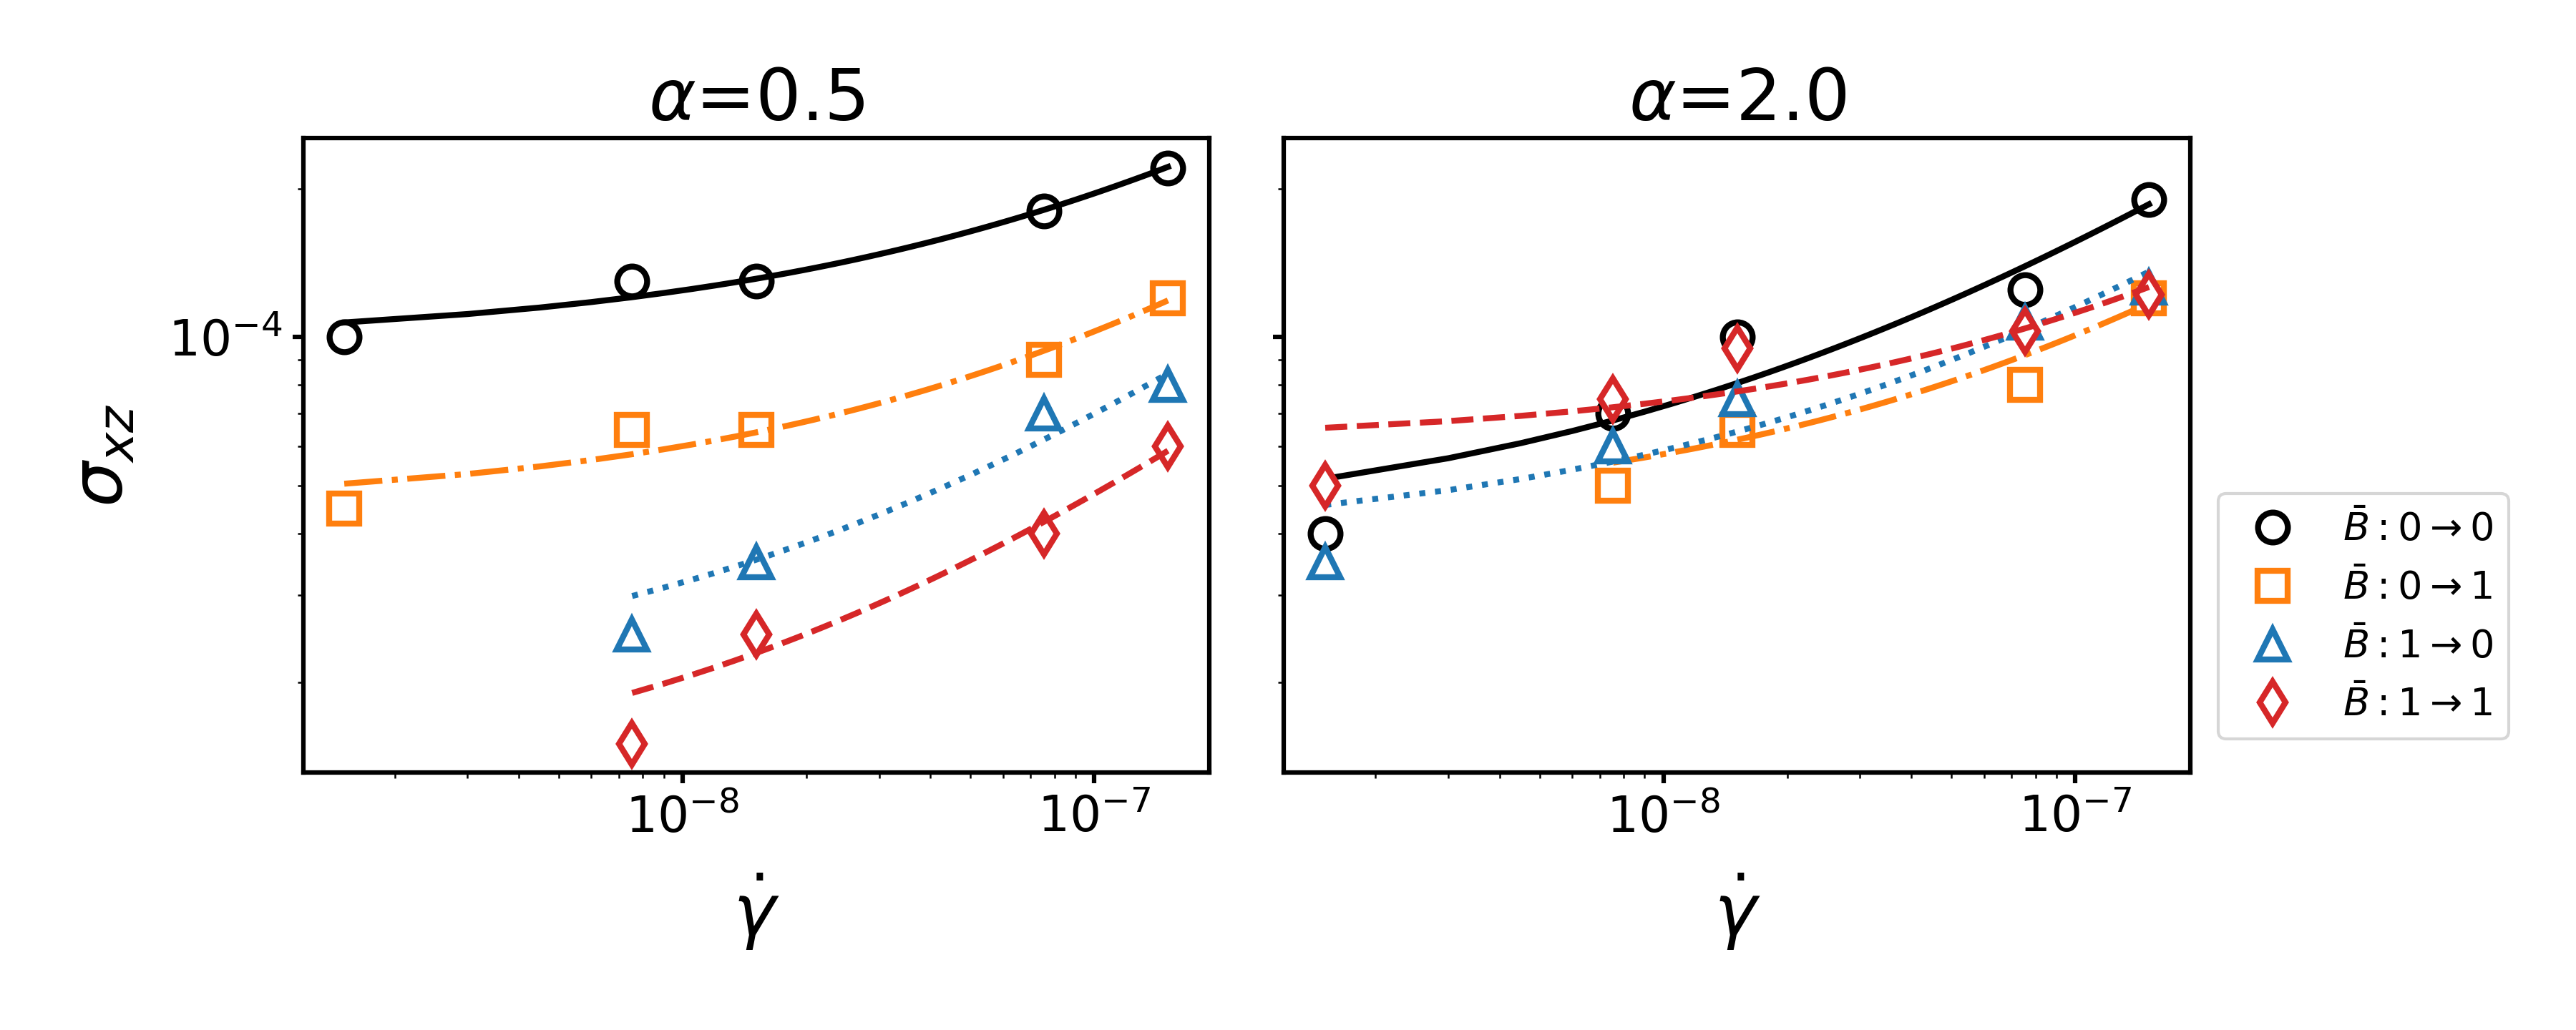
\includegraphics[scale=0.5]{../figures/results/paper3/stress_strain-all.png} 
    \caption{Fitting the experimental shear stress to the strain rate using the Herschel-Bulkley model. We characterize the bijels are 
             shear thinning in all cases and that the bijels become less shear thinning as the particle order increases. We also
             demonstrate that the particle ordering affects the yield stress differently for particles stabilized by oblate and 
             prolate particles.} 
    \label{fig:stress_strain} 
\end{figure}

Figure~\ref{fig:stress_strain} presents the shear stress $\sigma_{xz}$ as a function of shear rate $\dot{\gamma}$ for bijels stabilized by oblate ($\alpha = 0.5$) 
and prolate ($\alpha = 2.0$) ellipsoidal particles, fitted using the Herschel-Bulkley model. In both cases, the curves exhibit nonlinear scaling with $\dot{\gamma}$, 
confirming a non-Newtonian, shear-thinning response. For bijels stabilized by oblate particles, the stress-strain curves are more widely separated, indicating 
greater sensitivity to the initial microstructural configuration induced by magnetic field history. Specifically, increased orientational ordering—achieved through 
magnetic pre-alignment—correlates with a reduced yield stress, as observed by the downward shift of the stress curves. In contrast, bijels stabilized by prolate 
particles exhibit more closely clustered stress responses across different magnetic conditions, suggesting a reduced dependence on field history. Interestingly, 
for the prolate case, the stress response under persistent ordering ($\bar{B}:1 \rightarrow 1$) exceeds that of disordered systems, implying that aligned rod-like 
particles enhance interfacial resistance to shear. These trends highlight the contrasting rheological behaviors imparted by particle shape and the role of 
field-induced anisotropy in modulating mechanical response. Quantitative fit parameters obtained from the Herschel-Bulkley model are provided in 
Table~\ref{table:rheology_fit}.

\begin{table}[h!]
    \centering
    \renewcommand{\arraystretch}{1.5}  % Increases row height
    \begin{tabular}{||c c c c c||} 
     \hline
     Processing & $\alpha$ & $n$ & $K \frac{\Delta m (\Delta t)^{n-2}}{\Delta x} $ & $\sigma_{y} \frac{\Delta m}{\Delta x (\Delta t)^2}$ \\ [0.5ex] 
     \hline\hline
     $\bar{B}: 0 \rightarrow 0$ & 0.5 & 0.511 & 0.999 & $7.168 \cdot 10^{-5}$ \\ 
     \hline
     $\bar{B}: 0 \rightarrow 1$ & 0.5 & 0.579 & 0.944 & $4.008 \cdot 10^{-5}$ \\
     \hline
     $\bar{B}: 1 \rightarrow 0$ & 0.5 & 0.642 & 0.888 & $4.945 \cdot 10^{-5}$ \\
     \hline
     $\bar{B}: 1 \rightarrow 1$ & 0.5 & 0.637 & 0.914 & $1.715 \cdot 10^{-5}$ \\
     \hline
     $\bar{B}: 0 \rightarrow 0$ & 2 & 0.561 & 0.965 & $4.618 \cdot 10^{-5}$ \\
     \hline
     $\bar{B}: 0 \rightarrow 1$ & 2 & 0.609 & 0.944 & $4.101 \cdot 10^{-5}$ \\
     \hline
     $\bar{B}: 1 \rightarrow 0$ & 2 & 0.597 & 0.899 & $5.025 \cdot 10^{-5}$ \\
     \hline
     $\bar{B}: 1 \rightarrow 1$ & 2 & 0.606 & 0.885 & $6.435 \cdot 10^{-5}$ \\ [1ex] 
     \hline
    \end{tabular}
    \caption{Hershel Bulkley fit parameters for different processing conditions applied to bijels stabilized by ellipsoidal particles.}
    \label{table:rheology_fit}
\end{table}
 
The results presented in Table~\ref{table:rheology_fit} confirm that all bijel systems exhibit shear-thinning behavior, regardless of particle morphology or 
magnetic field history. The particle-shape-dependent differences in shear response observed in Figure~\ref{fig:stress_strain} are quantitatively reflected in 
the Hersche-Bulkley fit parameters, particularly in the yield stress $\sigma_y$ and flow index $n$. Notably, bijels synthesized with an applied magnetic field 
($\bar{B} = 1$) exhibit higher flow indices than those without, indicating a shift toward more Newtonian-like behavior under increased particle ordering. This 
trend is especially pronounced in bijels stabilized by oblate particles, where increased magnetic alignment leads to a progressive reduction in yield stress. 
In contrast, bijels stabilized by prolate particles show an opposite trend, with yield stress increasing alongside particle alignment and magnetic field 
application. These findings are consistent with earlier observations from Aim 1, which showed that magnetic fields promote local orientational ordering at the 
interface—enhancing ordering for prolate particles while reducing it for oblate particles. Prior studies have demonstrated that reduced local order in 
interfacial monolayers leads to structural buckling and early mechanical failure, whereas increased ordering enables more uniform stress distribution 
across particles, thereby enhancing resistance to deformation \cite{prakash_buckling_2024}.

\subsection{Shear induced particle rearrangement}

Given that magnetic fields can modify the local arrangement of ellipsoidal particles at fluid interfaces, understanding how this arrangement evolves under 
different processing conditions is essential for interpreting the mechanical 
behavior observed. In particular, the contrasting effects seen for prolate and oblate particles, where increased magnetic ordering leads to a larger
and smaller yield stress respectively. To quantitatively assess the local arrangement of particles at the interface, we compute the ensemble-averaged 
Steinhardt bond orientational order parameters $q_2$ and $q_6$. 
\cite{steinhardt_bond-orientational_1983, lechner_accurate_2008, mickel_shortcomings_2013}. These parameters characterize the local structural ordering by 
projecting the orientations of neighboring particles onto spherical harmonics of degree \(l\), and are defined as


\begin{equation}
q_l(i) = \left( \frac{4\pi}{2l+1} \sum_{m=-l}^{l} \left| \frac{1}{N(i)} \sum_{j=1}^{n(i)} Y_{lm}(\vec{r}_{ij}) \right|^2 \right)^{\frac{1}{2}} ,
\end{equation} 
%\TODO{update formula to the one actually used}

Here, \(n(i)\) denotes the number of nearest neighbors of particle \(i\), \(\vec{r}_{ij}\) is the vector connecting the centers of particles \(i\) and \(j\), 
and \(m\) is an integer ranging from \(-l\) to \(l\) that indexes the spherical harmonic components \(Y_{lm}\). Neighbor lists are typically defined using a 
fixed cutoff radius around each particle, identifying nearby particles as neighbors. We calculate the python package Freud to calculate the bond order parameters 
and use a Voronoi cell to determine the particle neighborhood rather than the standard distance criterion \cite{ramasubramani_freud_2020,mickel_shortcomings_2013}. 
The Voronoi-based method avoids the need for a predefined cutoff and yields more robust neighbor definitions, particularly in disordered systems. Bond 
orientational order parameters have been widely employed to study structural transitions in colloidal and ceramic systems, including crystallization, nucleation, 
and glass formation \cite{vagberg_glassiness_2011, besseling_three-dimensional_2007, schall_structural_2007, ozawa_jamming_2012}. $q_6$ is most commonly used 
to identify crystal structures by matching the calculated values to reference values for specific crystal structures such as fcc or hcp. We plot the change in 
$q_6$ of the microstructures as a function of the processing applied in Figure \ref{fig:q6_rheology_init}

\begin{figure} 
    \centering 
    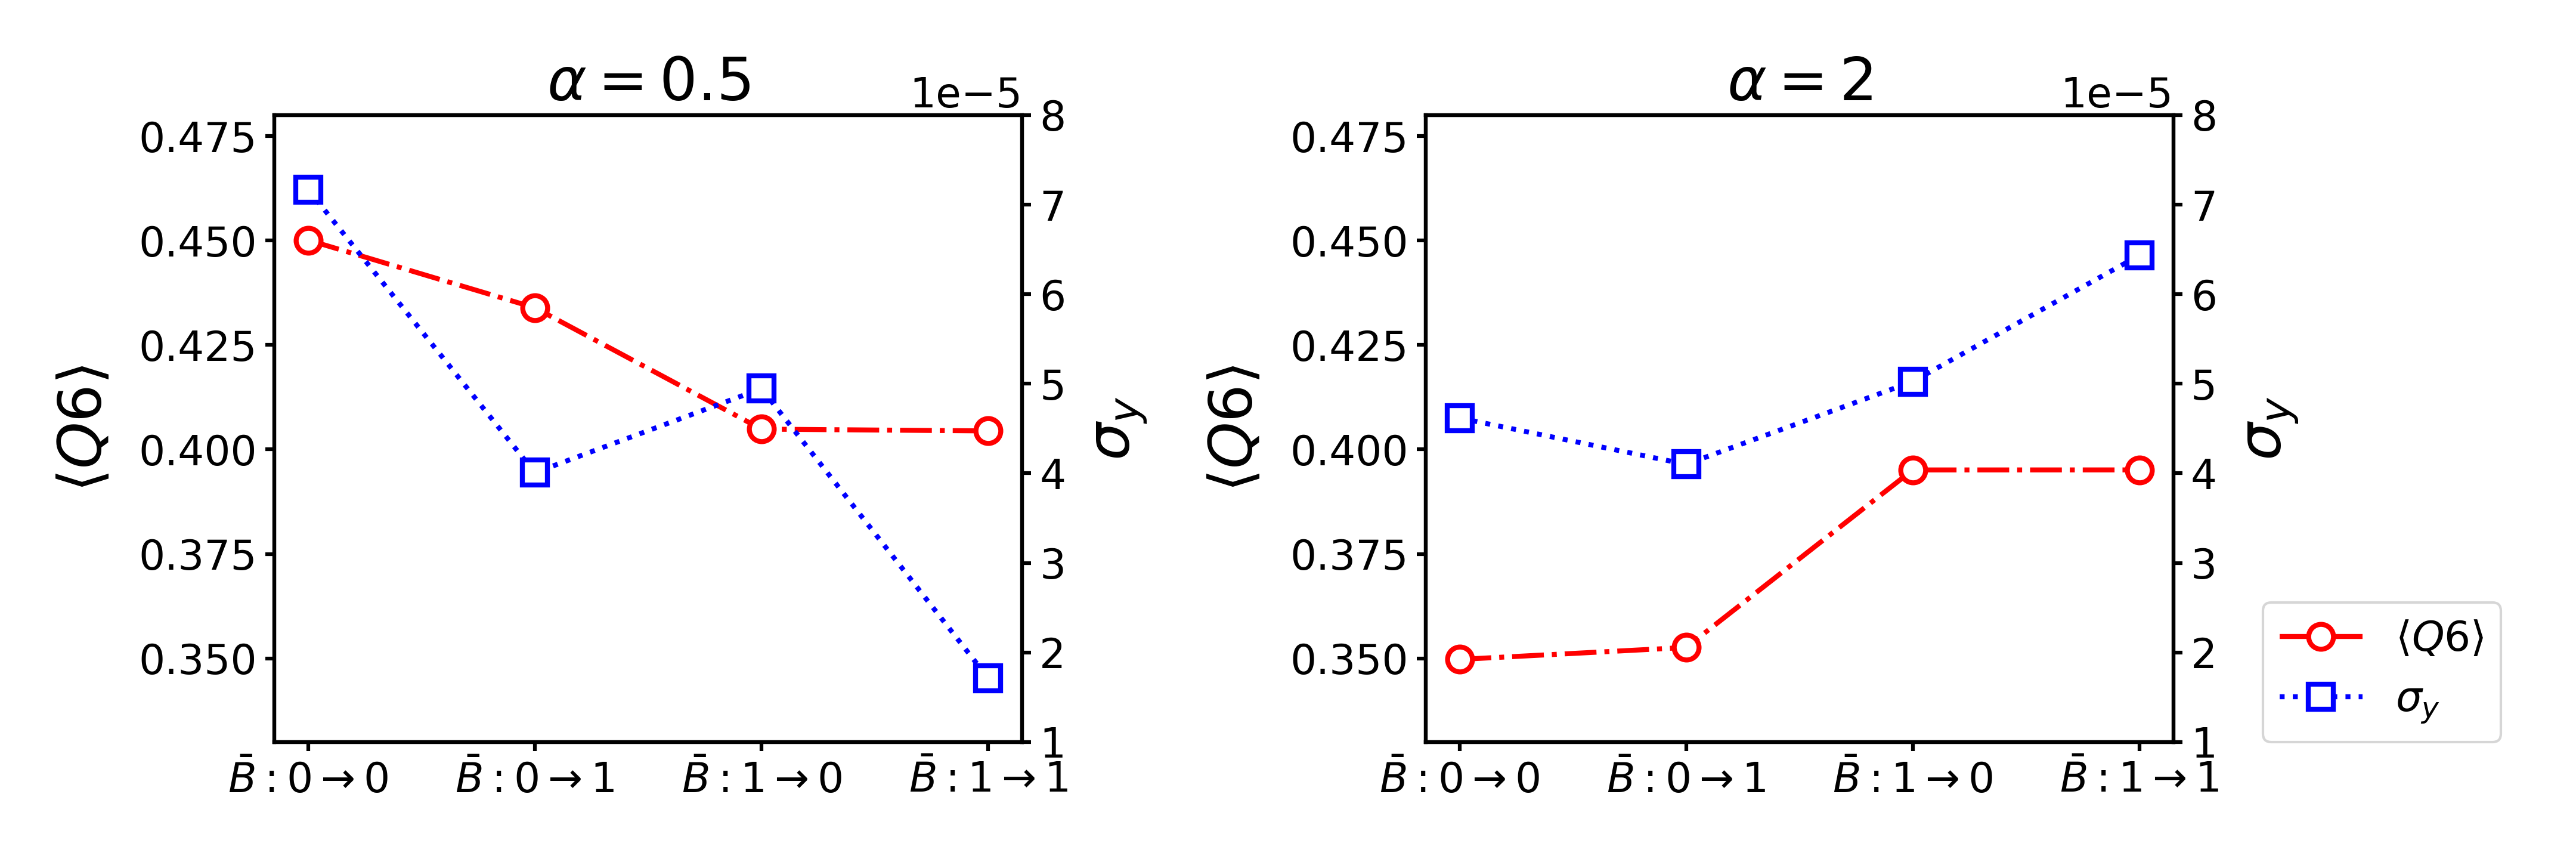
\includegraphics[scale=0.4]{../figures/results/paper3/Q6-start.png} 
    \caption{Plot of the relationship between the local particle order $\langle Q6 \rangle$ at the first timestep after initiation of shear and 
             yield stress ($\sigma_y$) in bijels across magnetic field histories for oblate 
             ($\alpha = 0.5$) and prolate ($\alpha = 2.0$) particle-stabilized systems.} 
    \label{fig:q6_rheology_init} 
\end{figure}

Figure~\ref{fig:q6_rheology_init} shows that for oblate particles (left panel), $\langle Q_6 \rangle$ decreases progressively with increasing magnetic alignment, 
indicating a loss of local hexagonal
order at the interface. This trend is accompanied by a reduction in yield stress, suggesting that disrupted interfacial packing compromises the bijel's 
ability to resist deformation. These findings align with prior observations that reduced local order facilitates monolayer buckling and structural failure 
under shear. In contrast, bijels stabilized by prolate particles display the opposite behavior, characterized as an increase in $\langle Q_6 \rangle$ with
the particle order field history, signifying enhanced local ordering, and this increase correlates with a substantial rise in yield stress. The positive 
coupling between local particle order and mechanical strength in prolate systems supports the hypothesis that nematic alignment reinforces the interfacial 
network, distributing stress more effectively under shear. Together, these results demonstrate a morphology-dependent link between magnetic field-induced 
ordering and rheological response. 

\subsection{Shear induced reorientation of particles}

Bonaccorso et al. identified that the spherical particle stabilizers in their bijel simulations oriented to the direction of shear before being
ejected from the interface. \cite{bonaccorso_shear_2020} Due to the shape of ellipsoidal particles, they adopt a preferred orientation which
maximizes the interface covered by the particle. \cite{davies_dipolar_2015, davies_interface_2014} Energy must be imparted to rotate the particles
out of the interface. Upon application of shear, the orientation of particles on the interface will be a function of the applied shear rate, 
applied magnetic field and the capillary forces of the interface on the particle. \cite{cao_modeling_2021, chhabra_drag_1999, brenner_stokes_1963, naga_capillary_2021}
Therefore, the degree of interface angle change observed can shed light onto the rheological 
differences of bijels stabilized by prolate and oblate particles as the shear stress determined is affected by the particle rotation on the interface. 

We analyzed the angle between each particles symmetry axis and the local interface normal by generating a mesh of the interface using the marching 
cubes algorithm and, for each particle, identified the nearest mesh vertex (excluding those beyond the length of the particle's long axis). We then calculated 
the angle $\psi$ between the particle orientation vector \(\hat{\vec{o}}_i\) and the local surface normal. The time evolution of the average interface
angle of all particles $\langle \psi \rangle$, calculated as a numerical average of $\psi$ for all particles, is shown in Figure~\ref{fig:interface_angle_shear}.

\begin{figure} 
    \centering 
    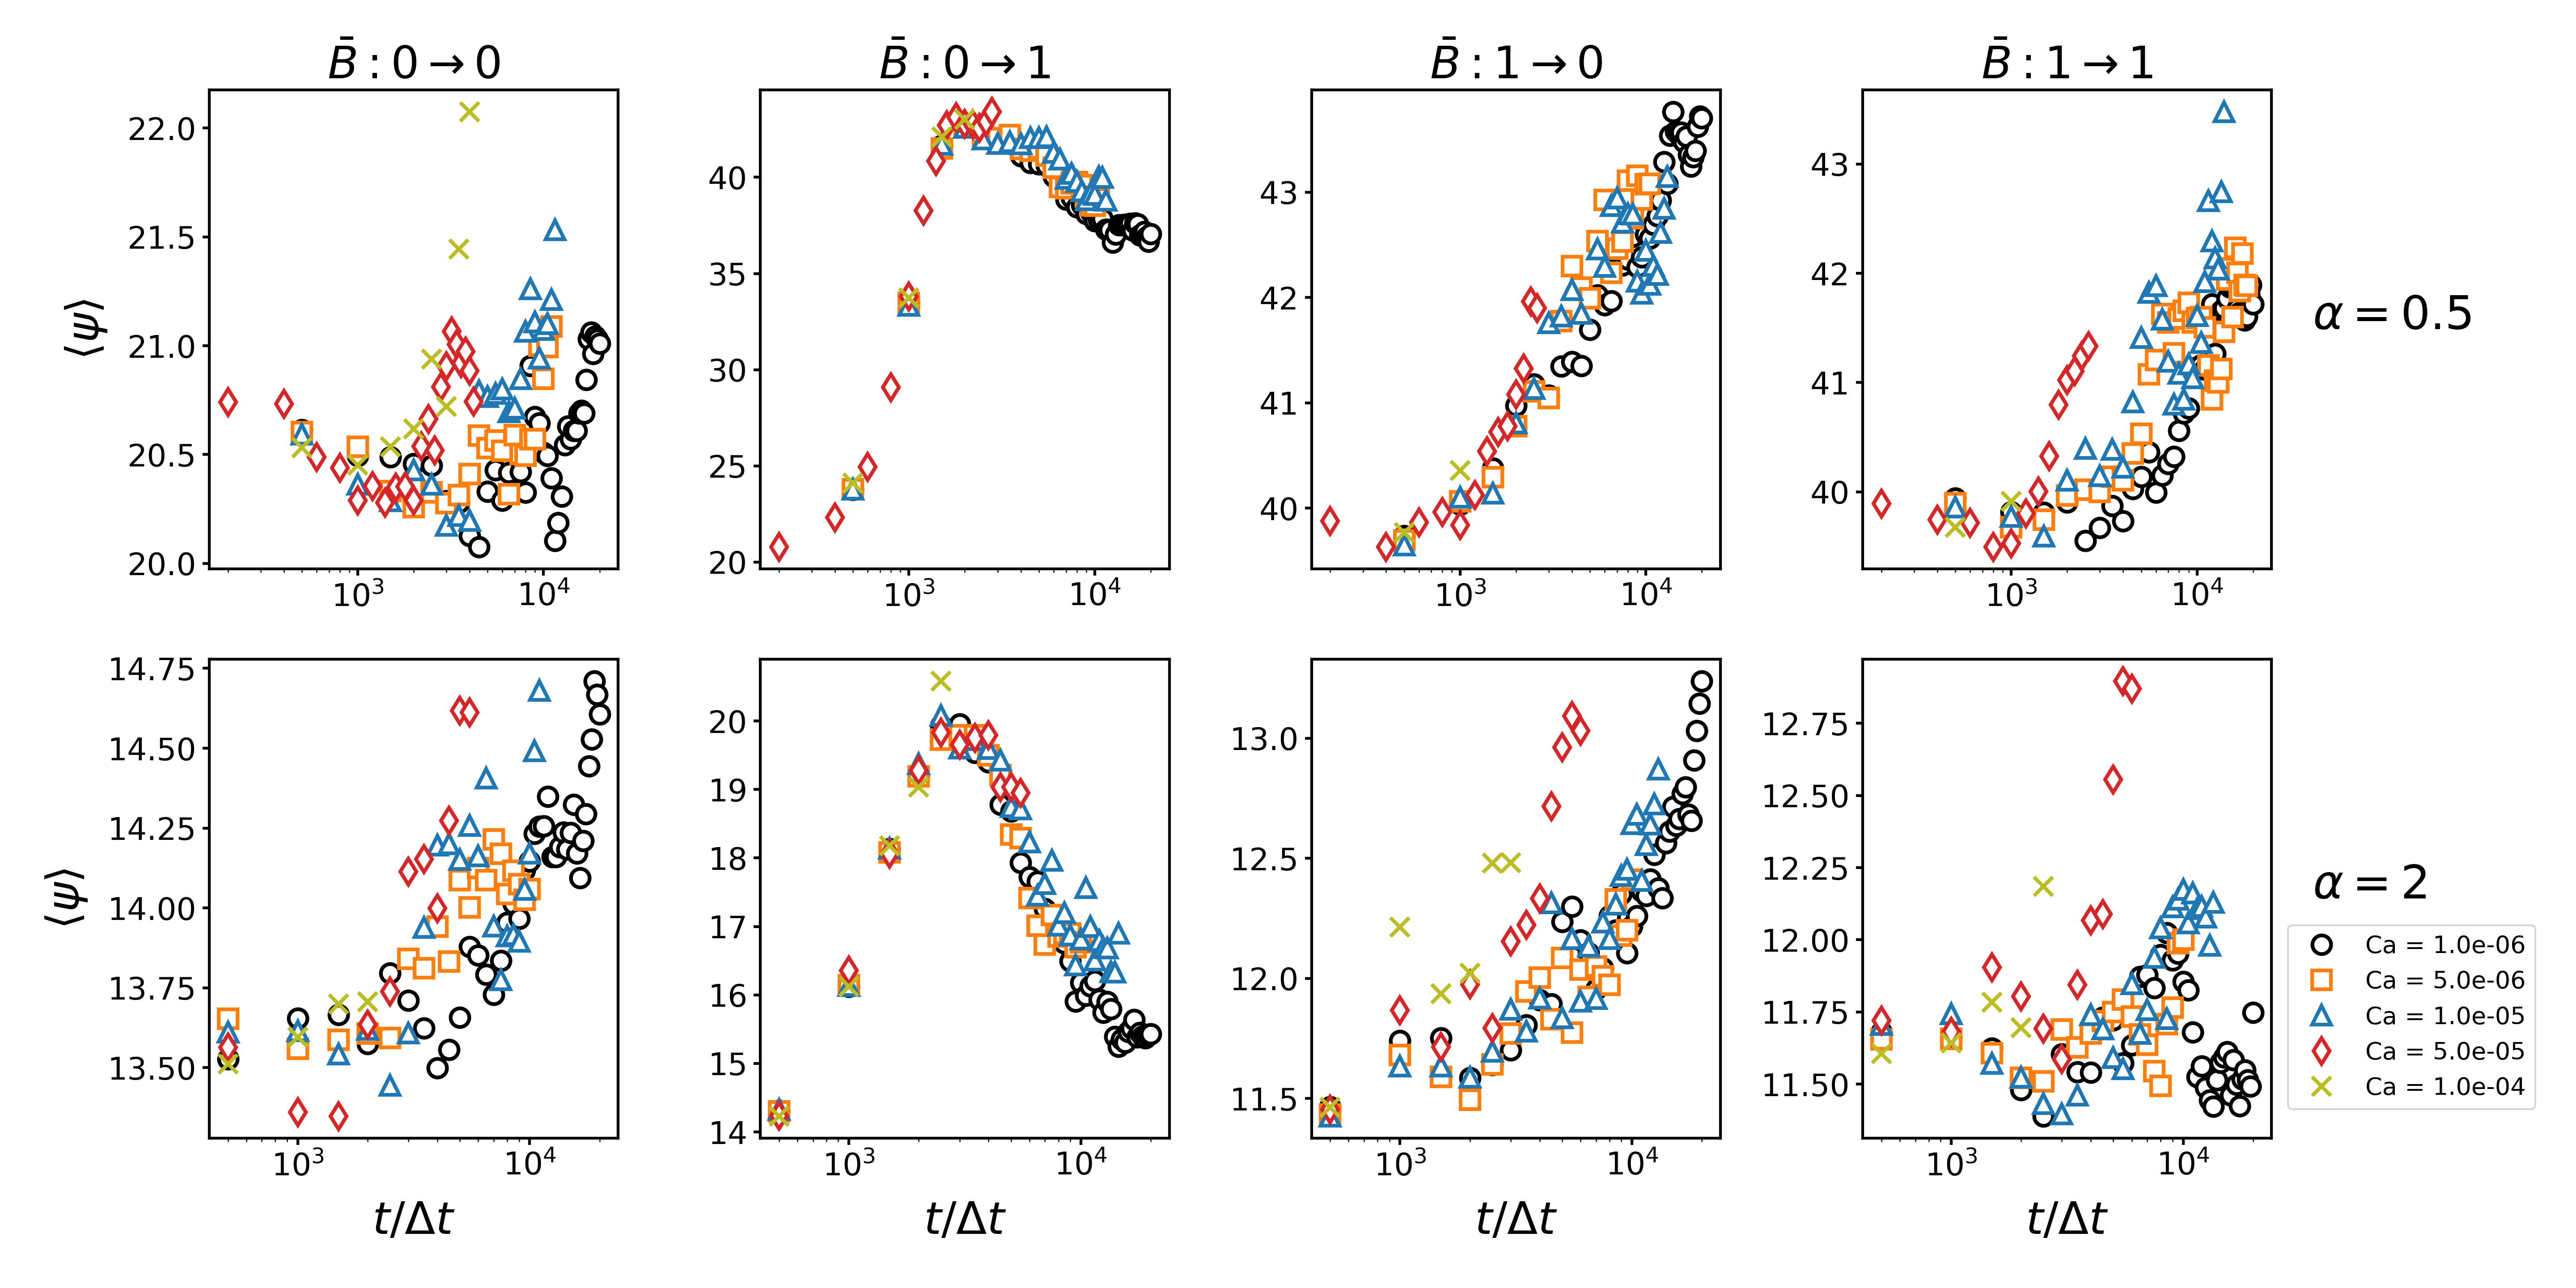
\includegraphics[scale=0.3]{../figures/results/paper3/psi-time_compare.png} 
    \caption{Comparisons of the interfacial angle of bijels stabilized by ellipsoidal particles as a function of 
             the applied shear rate at four different processing histories. We show that upon application of shear
             particles tilt out of the interface reduces the interfacial area stabilized. $\bar{B}: 0 \to 1$ shows 
             large variations in the interface angle.} 
    \label{fig:interface_angle_shear} 
\end{figure}

As shown in Figure~\ref{fig:interface_angle_shear}, the interface angle $\langle \psi \rangle$ generally increases over time across all cases, with the 
exception of the $\bar{B}: 0 \rightarrow 1$ condition. This indicates shear induced particle reorientation at the interface, indicating that particles are
being pulled out of the interface. The exception at $\bar{B}: 0 \rightarrow 1$ is consistent with the findings presented in Chapter~\ref{chapter:aim2}, where the 
observed behavior was attributed to particle reorientation toward the applied magnetic field. In all other cases, the gradual increase in $\langle \psi \rangle$ 
suggests that particles are progressively reorienting out of the interface under the influence of shear. For oblate particles initialized from bijel templates 
generated under $\bar{B} = 1$, the average initial interface angle is approximately 40°, indicating a pronounced tilt at the interface. As the tilt angle 
increases, the energy barrier to rotate a particle further out of the interface decreases, leading to reduced hydrodynamic drag and, consequently, lower 
effective viscosity. In contrast, the difference in initial interface angle between field- and non-field-aligned bijels stabilized by prolate particles 
is much smaller—approximately 13.5° and 11.5°, respectively. This smaller variation helps explain the more modest changes in rheological response observed 
in prolate systems, compared to the more pronounced field-dependent behavior in oblate particle-stabilized bijels.

\section{Conclusions}

In this study, we investigated the rheological behavior of bijels stabilized by magnetically responsive ellipsoidal particles subjected to constant shear. 
In systems like solvent transfer-induced phase separation (STrIPS) and volatile-induced phase separation (VIPS), rheology plays a key role in determining the
microstructure and morphology of the bijel. The presence of anisotropic particles and external magnetic fields further complicates this behavior 
by altering interfacial structure. To systematically probe these effects, we employed a hybrid Lattice Boltzmann-Molecular Dynamics (LBM-MD) simulation 
framework to evaluate how particle shape, magnetic field history, and interfacial microstructure jointly influence the flow response of bijels. 
Four magnetic processing pathways were considered—ranging from fully unordered systems to those with persistent particle alignment—across a range of 
shear capillary numbers. By fitting the resulting stress-strain data to a Herschel-Bulkley model, we characterized the yield stress and degree of shear 
thinning for each configuration.

Our results show that bijels exhibit non-Newtonian, shear-thinning behavior regardless of processing history or particle morphology. However, both yield stress 
and flow index are highly sensitive to the initial degree of particle alignment at the interface. Bijels stabilized by oblate particles demonstrated substantial 
variation in yield stress across magnetic field histories, with increased ordering correlating with a reduction in stress response. Conversely, bijels stabilized 
by prolate particles exhibited more consistent rheological behavior, with yield stress increasing in response to magnetic alignment. Systems initialized with 
fully ordered structures ($\bar{B}:1 \rightarrow 1$) showed the highest resistance to flow for prolate particles, while oblate systems in the same condition 
yielded more readily.

To interpret these rheological differences, we analyzed both local structural ordering (via the Steinhardt $Q_6$ parameter) and particle orientation relative to 
the interface. Increased magnetic alignment in prolate systems led to higher $Q_6$ values and lower interface angles, indicating that particles remained 
well-anchored to the interface. This ordering enhanced stress distribution, leading to higher yield stress. In contrast, oblate particles 
tended to tilt further from the interface when aligned, as confirmed by elevated interface angles and decreased $Q_6$, making the monolayer more susceptible to 
shear-induced buckling and collapse. The increased interface angle of oblate particles after application of a field reduces the torque necessary to rotate particles
out of the interface, resulting in the larger differences in shear stress calculated for bijels stabilized with oblate particles.

These findings highlight the interplay between particle anisotropy, interfacial order, and external magnetic fields in tuning the mechanical properties of bijels. 
By modulating particle alignment through magnetic stimuli, it is possible to tailor the yield stress and flow behavior of these materials—a property of potential 
interest in fields such as soft robotics, drug delivery, and responsive templating. Moreover, the contrast in behavior between oblate and prolate particles 
underscores the importance of shape-specific design in engineering structured fluids. In the next chapter, we extend this investigation to consider dynamic or 
transient shear regimes and explore the reversibility of these structural transitions under cyclic loading and field modulation.